\chapter{Hybrid-Cloud-Architektur}
\label{cha:hybrid_cloud_architektur}

Im folgenden Kapitel wird eine Hybrid-Cloud-Architektur entwickelt. Dafür wird, wie in Abbildung
\ref{fig:architektur_uebersicht} auf Seite \pageref{fig:architektur_uebersicht} zu sehen, eine dauerhafte Verbindung
zwischen dem Netzwerk der Cloud-Infrastruktur und dem lokalen Netzwerk des Mainframes hergestellt. Diese Verindung soll
über mehrere Kommunikationskanäle verfügen, um verschiedene Programme miteinander zu verbinden.

Anschließend soll es in der Cloud eine Konfigurationsansicht geben um Ressourcen auf dem Mainframe zu verwalten. Dazu
gehört neben dem Erstellen dieser auch das Starten, Stoppen und Löschen. Die Ansicht soll außerdem Informationen über
die einzelnen Ressourcen und das Gesamtsystem anzeigen und auswerten können.

Des Weiteren wird eine Möglichkeit gefunden, wie Quellcode, welcher entweder in der Cloud oder in einem lokalen RTC
gespeichert ist, gebaut und in der Cloud oder auf dem Mainframe installiert und ausgeführt werden kann.

Einem Entwickler soll es in Zukunft möglich sein, seinen Quellcode lokal auf einem Mainframe oder in einer Cloud zu
verwalten, anschließend Ressourcen sowohl in der Cloud als auch auf dem Mainframe bereitzustellen, seinen Quellcode zu
bauen und auf beiden Systemen einzurichten.

Auch soll es dem Entwickler möglich sein, ein Segment seiner Anwendung auf dem lokalen Mainframe und das andere in der
Cloud bereitzustellen. Somit können bestehende Anwendungen weiterhin genutzt werden. Eine Kommunikation der beiden
Segmente vorausgesetzt.

\begin{figure}[h]
  \centering
    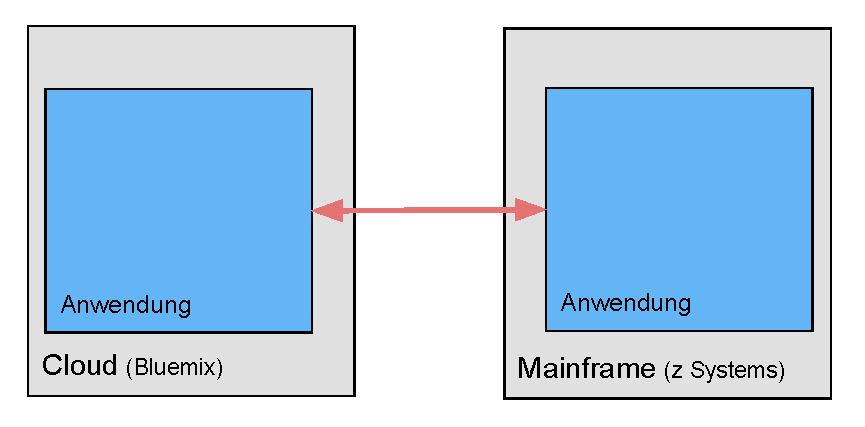
\includegraphics[scale=0.5]{images/kapitel_3/architektur_uebersicht.pdf}
  \caption{Schematische Darstellung der Hybrid-Cloud-Architektur}
  \label{fig:architektur_uebersicht}
\end{figure}